\documentclass{acm_proc_article-sp}
\usepackage{textcomp}
\usepackage{color}
\usepackage{hyperref}

\begin{document}

\title{Poster:Re-designing Drainage System to Solve Water Logging Using Cloud-Based Mobile Application}
%
% You need the command \numberofauthors to handle the 'placement
% and alignment' of the authors beneath the title.
%
% For aesthetic reasons, we recommend 'three authors at a time'
% i.e. three 'name/affiliation blocks' be placed beneath the title.
%
% NOTE: You are NOT restricted in how many 'rows' of
% "name/affiliations" may appear. We just ask that you restrict
% the number of 'columns' to three.
%
% Because of the available 'opening page real-estate'
% we ask you to refrain from putting more than six authors
% (two rows with three columns) beneath the article title.
% More than six makes the first-page appear very cluttered indeed.
%
% Use the \alignauthor commands to handle the names
% and affiliations for an 'aesthetic maximum' of six authors.
% Add names, affiliations, addresses for
% the seventh etc. author(s) as the argument for the
% \additionalauthors command.
% These 'additional authors' will be output/set for you
% without further effort on your part as the last section in
% the body of your article BEFORE References or any Appendices.
 \newcommand*{\myaffaddr}[1]{#1} % No op here. Customize it for different styles.
 \newcommand*{\myaffmark}[1][*]{\textsuperscript{#1}}
\numberofauthors{3} 
\author{
Sadia Sharmin\myaffmark[1], 
Mitrasree Deb\myaffmark[2], 
Dipto Borua \myaffmark[3]\\
 \myaffaddr{Department of Computer Science and Engineering}\\
 \myaffaddr{Bangladesh University of Engineering and Technology}\\
 \email{\myaffmark[1]sadiasharmin@cse.buet.ac.bd, \myaffmark[2]mitrasree091@gmail.com,
\myaffmark[3]diptoborua9@gmail.com }\\
 }
%  in this sample file, there are a *total*
% of EIGHT authors. SIX appear on the 'first-page' (for formatting
% reasons) and the remaining two appear in the \additionalauthors section.
%
%\author{
% You can go ahead and credit any number of authors here,
% e.g. one 'row of three' or two rows (consisting of one row of three
% and a second row of one, two or three).
%
% The command \alignauthor (no curly braces needed) should
% precede each author name, affiliation/snail-mail address and
% e-mail address. Additionally, tag each line of
% affiliation/address with \affaddr, and tag the
% e-mail address with \email.
%
% 1st. author
% \alignauthor
% Mitrasree Deb\\
%        \affaddr{Undergraduate Student}\\
%        \affaddr{Department of Computer Science \& Engineering}\\
%        \affaddr{Bangladesh University of Engineering \& Technology}\\
%        \affaddr{Dhaka-1000}\\
%        %\affaddr{telephone number, incl. country code}
%        \email{mitrasree091@gmail.com}
% % 2nd. author
% \alignauthor
% Dipto Borua\\
%        \affaddr{Undergraduate Student}\\
%        \affaddr{Department of Computer Science \& Engineering}\\
%        \affaddr{Bangladesh University of Engineering \& Technology}\\
%        \affaddr{Dhaka-1000}\\
%        %\affaddr{telephone number, incl. country code}
%        \email{diptoborua9@gmail.com}
% % 3rd. author
% %\alignauthor Lars Th{\o}rv{\"a}ld\titlenote{This author is the
% %one who did all the really hard work.}\\
% %       \affaddr{The Th{\o}rv{\"a}ld Group}\\
% %       \affaddr{1 Th{\o}rv{\"a}ld Circle}\\
% %       \affaddr{Hekla, Iceland}\\
% %       \email{larst@affiliation.org}
% %\and  % use '\and' if you need 'another row' of author names
% %% 4th. author
% '\and'
% \alignauthor 
% Sadia Sharmin\\
%         \affaddr{Assistant Professor}\\
%         \affaddr{Department of Computer Science \& Engineering}\\
%         \affaddr{Bangladesh University of Engineering \& Technology}\\
%         \affaddr{Dhaka-1000}
%         \email{sadiasharmin@cse.buet.ac.bd}
%% 5th. author
%\alignauthor Sean Fogarty\\
%       \affaddr{NASA Ames Research Center}\\
%       \affaddr{Moffett Field}\\
%       \affaddr{California 94035}\\
%       \email{fogartys@amesres.org}
%% 6th. author
%\alignauthor Charles Palmer\\
%       \affaddr{Palmer Research Laboratories}\\
%       \affaddr{8600 Datapoint Drive}\\
%       \affaddr{San Antonio, Texas 78229}\\
%       \email{cpalmer@prl.com}
%}
% There's nothing stopping you putting the seventh, eighth, etc.
% author on the opening page (as the 'third row') but we ask,
% for aesthetic reasons that you place these 'additional authors'
% in the \additional authors block, viz.
%\additionalauthors{Additional authors: John Smith (The Th{\o}rv{\"a}ld Group,
%email: {\texttt{jsmith@affiliation.org}}) and Julius P.~Kumquat
%(The Kumquat Consortium, email: {\texttt{jpkumquat@consortium.net}}).}
%\date{30 July 1999}
% Just remember to make sure that the TOTAL number of authors
% is the number that will appear on the first page PLUS the
% number that will appear in the \additionalauthors section.

\maketitle

\section{Introduction}

Water logging has been disrupting livelihoods of about one million people in Bangladesh during past two decades. The capital city Dhaka faces extensive water logging during the monsoon (May to October) as a regular  phenomenon due to fast and uncontrolled urbanization. This is creating adverse social,physical,economic and environmental impacts in the life and living in Dhaka. Not only that,this problem has also been persistent in some big cities of India (i.e,Kolkata)~\cite{royseasonal}.\\In this work, we propose a cloud-based mobile solution to redesign a city\textquotesingle s drainage system to solve the water logging problem. For our case study, we chose Dhaka as our first city to try the proposed application.

\section{Background and Related Work}

Earlier there has been extensive research on water logging in Dhaka city ~\cite{neelopal2010water}.
% \\Another case study inclined to water logging along with drainage system proposal has been carried out by two authors~\cite{anisha2014case}.
These studies have a brief description on the current situation of water logging but there is still the need of a solution. 
for making this problem not persistent anymore.Our proposed solution has the application of user-data along with an algorithmic approach.
% 
\section{Approach and Uniqueness}

 Our proposed solution leverages proper estimation of water clogged upon which measures can be taken alongside re-designing the drainage system all over the city.


\textbf{Step 1:} We have collected data of water logging events from the user survey via mobile application. Data include the height of logged water as well as the garbage level at different points of the city. From these data,we can almost precisely measure the amount of extra water (in volume) that needs to be extracted from a particular area. These areas are determined by using convex hull algorithm.
\begin{figure}[ht!]
\centering
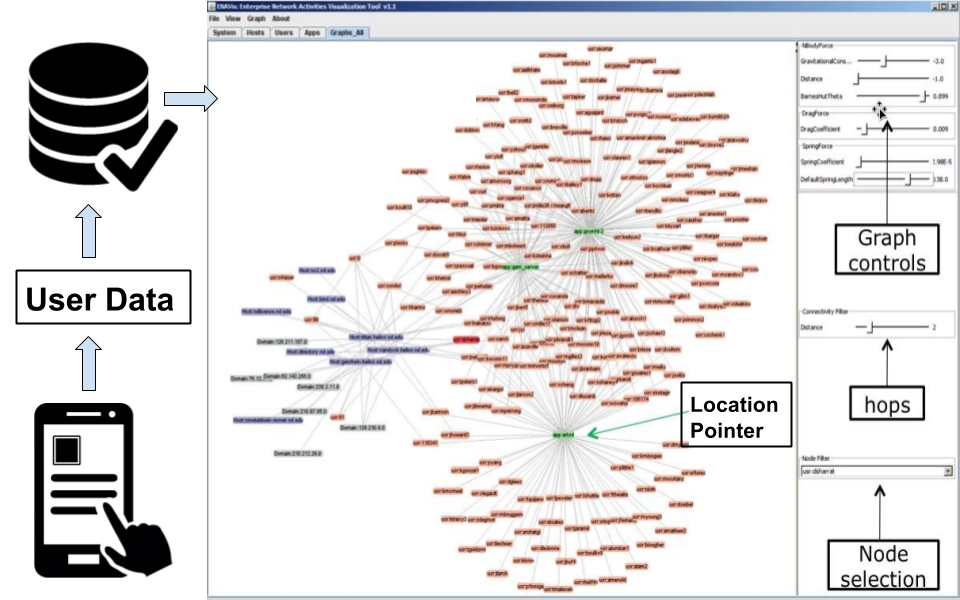
\includegraphics[width=1.0\linewidth]{flow.png}
\caption{Process of obtaining data and producing pipeline design}
\end{figure}


\textbf{Step 2:} The Govt. has a placement map of pipelines of the city with proper measurements (i.e. length, radius etc.). To accommodate all the water in a certain pipeline,the change in the pipeline measurements is calculated. 

\textbf{Step 3:} To remove the maximum amount of water at an optimal time, Ford-Fulkerson's maximum flow algorithm is applied. 

% \textbf{Step:4} Data yielding from the calculations provide us with a plan for:

% \ i. Properly measured pipelines with maximum capacity and minimum cost.\\
% \ ii. Extracting the extra water (from calculation) to places with less water logging.


% \subsection{Uniqueness}

% The water logging problem has been a burning issue now-a-days.In spite of carrying out numerous research and campaigns,it still persists in the city causing sufferings to the people specially those who live in low-lying areas.Our approach is unique as it gives a practical solution based on the current situation.It is not only just a statistics rather it has implementation in real-life.

\section{Results and Contributions}

Users can report different incidents of logging categorized on areas. Around 50 users of 3 to 4 different locations,used our application.  We wish to produce a cross-referencing Google map by crowd-sourcing~\cite{hara2014tohme} user data to formulate actual flooded area (with the help of image processing). We also planned to accumulate regression lines depending of different seasons and place them accordingly in the map.

% \begin{figure}[ht!]
% \centering
% 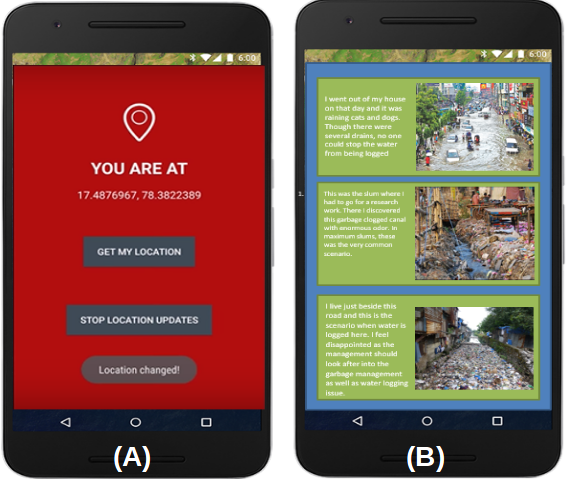
\includegraphics[width=1.0\linewidth]{App.png}
% \caption{Figure02 :(A)Area detection via GPS., (B)User Reports with uploaded figures.}
% \end{figure}
 

%\subsection{Results}

%Provide an overview of results.  Use tables or figures as appropriate.  Place Tables/Figures/Images in text as close to the reference as possible, typically at the top of a column (see Figure~\ref{fig:myfig}).  
% The location based data collection is done via the GPS location in the mobile application.After the collection of data,they are plotted into a graph.Ford-Fulkerson's maximum flow algorithm yields the graph to a proper pipeline design for a specific area accordingly.


% \begin{figure}[ht!]
% \centering
% 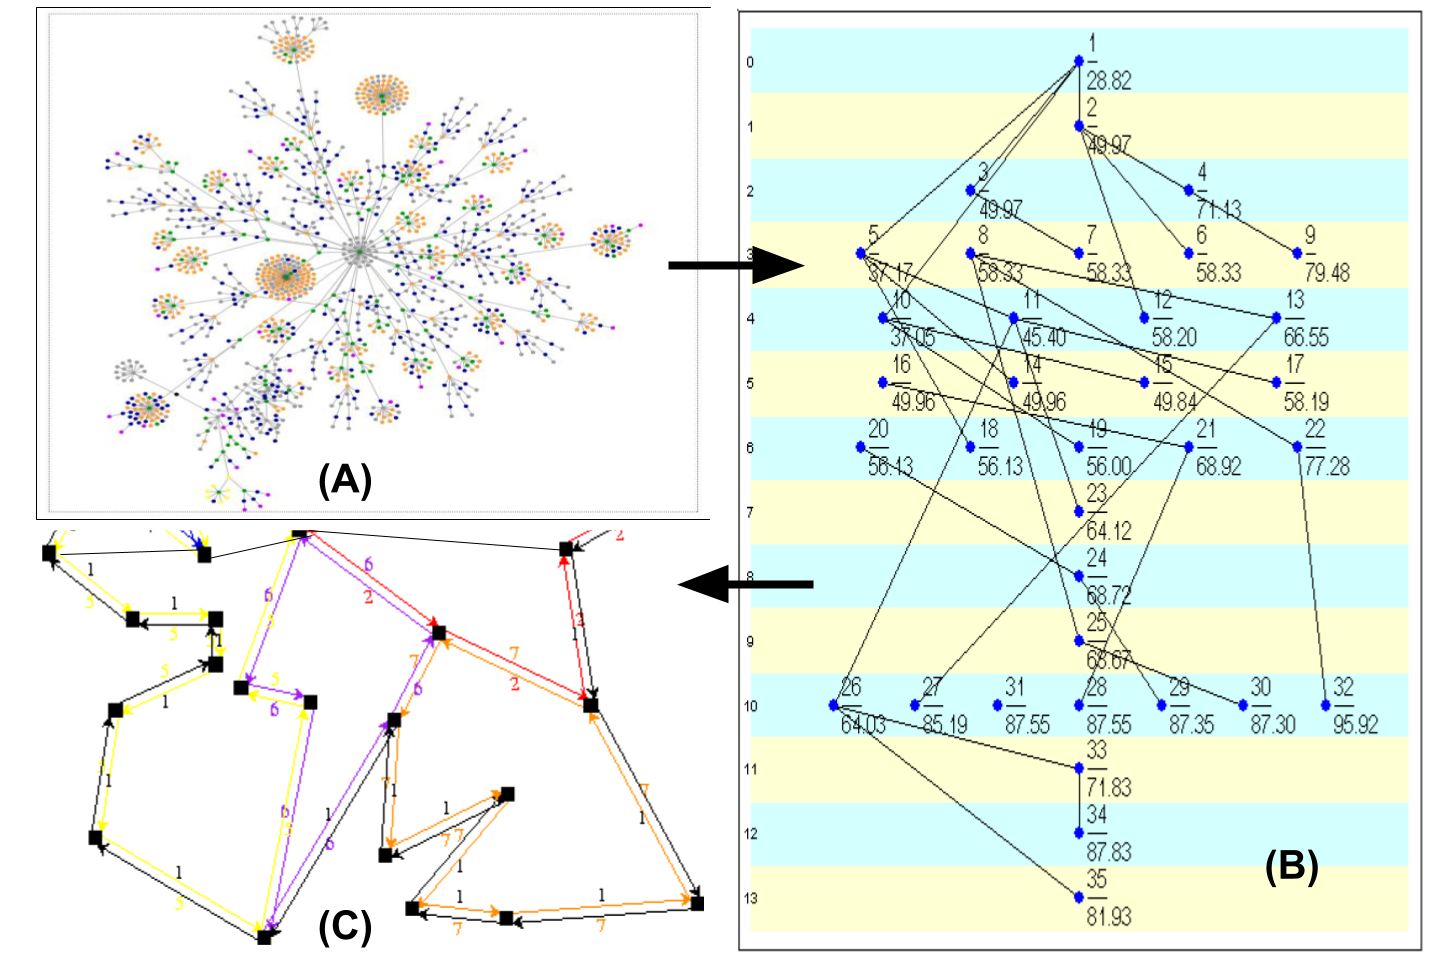
\includegraphics[width=1.1\linewidth]{data1.png}
% \caption{Figure03:(A)User data based on location,(B)Graph of points associated with values,(C)Pipeline design}
% \end{figure}

%\begin{figure}
%\centering
%\epsfig{file=process}
%\caption{A sample black and white graphic (.pdf format).}
%\label{fig:myfig}
%\end{figure}

%\begin{table}
%\centering
%\caption{Table}
%\begin{tabular}{|c|c|c|c|} 
%\hline
%\textbf{Graphics} & \textbf{Top} & \textbf{In-between} & \textbf{Bottom} \\ \hline
%Tables & End & Last & First \\ \hline
%Figures & Good & Similar & Very well \\ \hline
%\end{tabular}
%\end{table}

% \subsection{Contributions}

% The contributions of our work are:

% \begin{itemize}
% \item{Our algorithmic approach is feasible and much more optimized.}
% \item{The mobile application is user friendly and helps to obtain location based data using GPS.}
% \item{The data analysis process is much more inclined towards a better optimized processing of data.}
% \end{itemize}

% \section{Future Plans}

% As per our progress,we wish to produce a cross-referencing Google map by crowd-sourcing~\cite{hara2014tohme} user data to formulate actual flooded area (with the help of image processing).We have plans to accumulate regression lines depending of different seasons and place them accordingly in the map.

% The following two commands are all you need in the
% initial runs of your .tex file to
% produce the bibliography for the citations in your paper.

\bibliographystyle{plain}

\bibliography{sigproc}  % sigproc.bib is the name of the Bibliography in this case

%\section{References}

 %[1] Dhaka\textquotesingle s Chronic Water Logging Problem\\
  %\url{http://www.theindependentbd.com/post/4829}\\

% You must have colora proper ".bib" file
%  and remember to run:
% latex bibtex latex latex
% to resolve all references

\balancecolumns
\end{document}
